% Going off the Thesis guidelines available here: http://www.lboro.ac.uk/students/welcome/research/codes-of-practice/appendices/
% A4 paper size selected, default is 11pt font, to change to 12pt use [a4paper, 12pt] as option to documentclass
\documentclass[a4paper]{report}

% Some useful packages for including images, colored font, etc.
\usepackage[dvips]{graphicx}
\graphicspath{{Figures/}}

\makeatletter
\def\maxwidth{\ifdim\Gin@nat@width>\linewidth\linewidth\else\Gin@nat@width\fi}
\def\maxheight{\ifdim\Gin@nat@height>\textheight\textheight\else\Gin@nat@height\fi}
\makeatother
\setkeys{Gin}{width=\maxwidth,height=\maxheight,keepaspectratio}
\usepackage{amssymb,amsmath}
\usepackage{longtable}
\usepackage{booktabs}

\usepackage{listings}
\usepackage{xcolor}
 
\definecolor{codegreen}{rgb}{0,0.6,0}
\definecolor{codegray}{rgb}{0.5,0.5,0.5}
\definecolor{codepurple}{rgb}{0.58,0,0.82}
\definecolor{backcolour}{rgb}{0.95,0.95,0.92}
 
\lstdefinestyle{mystyle}{
    backgroundcolor=\color{backcolour},   
    commentstyle=\color{codegreen},
    keywordstyle=\color{magenta},
    numberstyle=\tiny\color{codegray},
    stringstyle=\color{codepurple},
    basicstyle=\ttfamily\footnotesize,
    breakatwhitespace=false,         
    breaklines=true,                 
    captionpos=b,                    
    keepspaces=true,                 
    numbers=left,                    
    numbersep=5pt,                  
    showspaces=false,                
    showstringspaces=false,
    showtabs=false,                  
    tabsize=2
}
 
\lstset{style=mystyle}

\usepackage[numbers]{natbib}

\usepackage{color}
\usepackage{url}
% Used for subfigures
\usepackage{subcaption}
% Used for landscape pages
\usepackage{pdflscape}
% Used for hyper-links in contents, etc.
\usepackage[hidelinks]{hyperref}
\hypersetup{
    linktoc=all
}

% Global bibliography style
\bibliographystyle{plain}

% Set margins in all document to 3.5cm as per guidelines for binding
\usepackage[includeheadfoot,margin=3.5cm]{geometry}

% Used to including pdf files within pages
% use [draft] as option to output empty spaces rather than rendering all pages (useful when including lots of pdfs)
\usepackage{pdfpages}

% Used to produce headers and footers
\usepackage{fancyhdr}
\pagestyle{fancyplain}

% Used for removing title in bibliography sections
\usepackage{titlesec}

% Used to generate lists of abbreviations
\usepackage{nomencl}
\makenomenclature 
\renewcommand{\nomname}{List of Abbreviations} 

% To have a separate bibliography per Chapter uncomment this line
% See Introduction/Introduction.tex for example how to include the bibliography
%\usepackage{chapterbib}

% Line spacing defined at 1 and a half. I know it says 1.3 but its 1 and a half.
\linespread{1.3}

% Setup headers and footers
\fancyhf{}
\lhead{\leftmark}
% Center on all pages
% \fancyhead[C]{---Draft---}
% Page number placed on right side on odd pages and left side on even pages
\fancyfoot[RO, LE] {\thepage}


\begin{document}

% Give \subsubsection numbers
\setcounter{secnumdepth}{4}

% Title, Author, Abstract, Acknowledgement, Table of Content, List of Figures, List of Tables and List of Abbreviations
% Front matter of the Thesis
% Title page
% Loughborough University Thesis Access Form
% Loughborough University Certificate of Originality
% Abstract
% Acknowledgements
\title{\bf Mobile Robot}

\author{by\\Zhihao DAI\\
Keli ZHANG\\
Changrong CHEN\\
Suraj Kumar\\
Yihang AI\\
\\
{\bf COP518 Robotics \& Intelligent Systems}\\
{\bf Coursework Report}\\
\\
Loughborough University\\
\\
\copyright
\hspace{1 dd} Zhihao DAI 2020\\
\\
Feb. 2020
}
\date{} % Used to remove date from title so it can be set at any date rather than the current date

\maketitle

% Set page numbers to roman numerals for front matter
\pagenumbering{roman}

% % PDF exports of Word Documents available (Exported August 2012)
% % Thesis Access Form
% 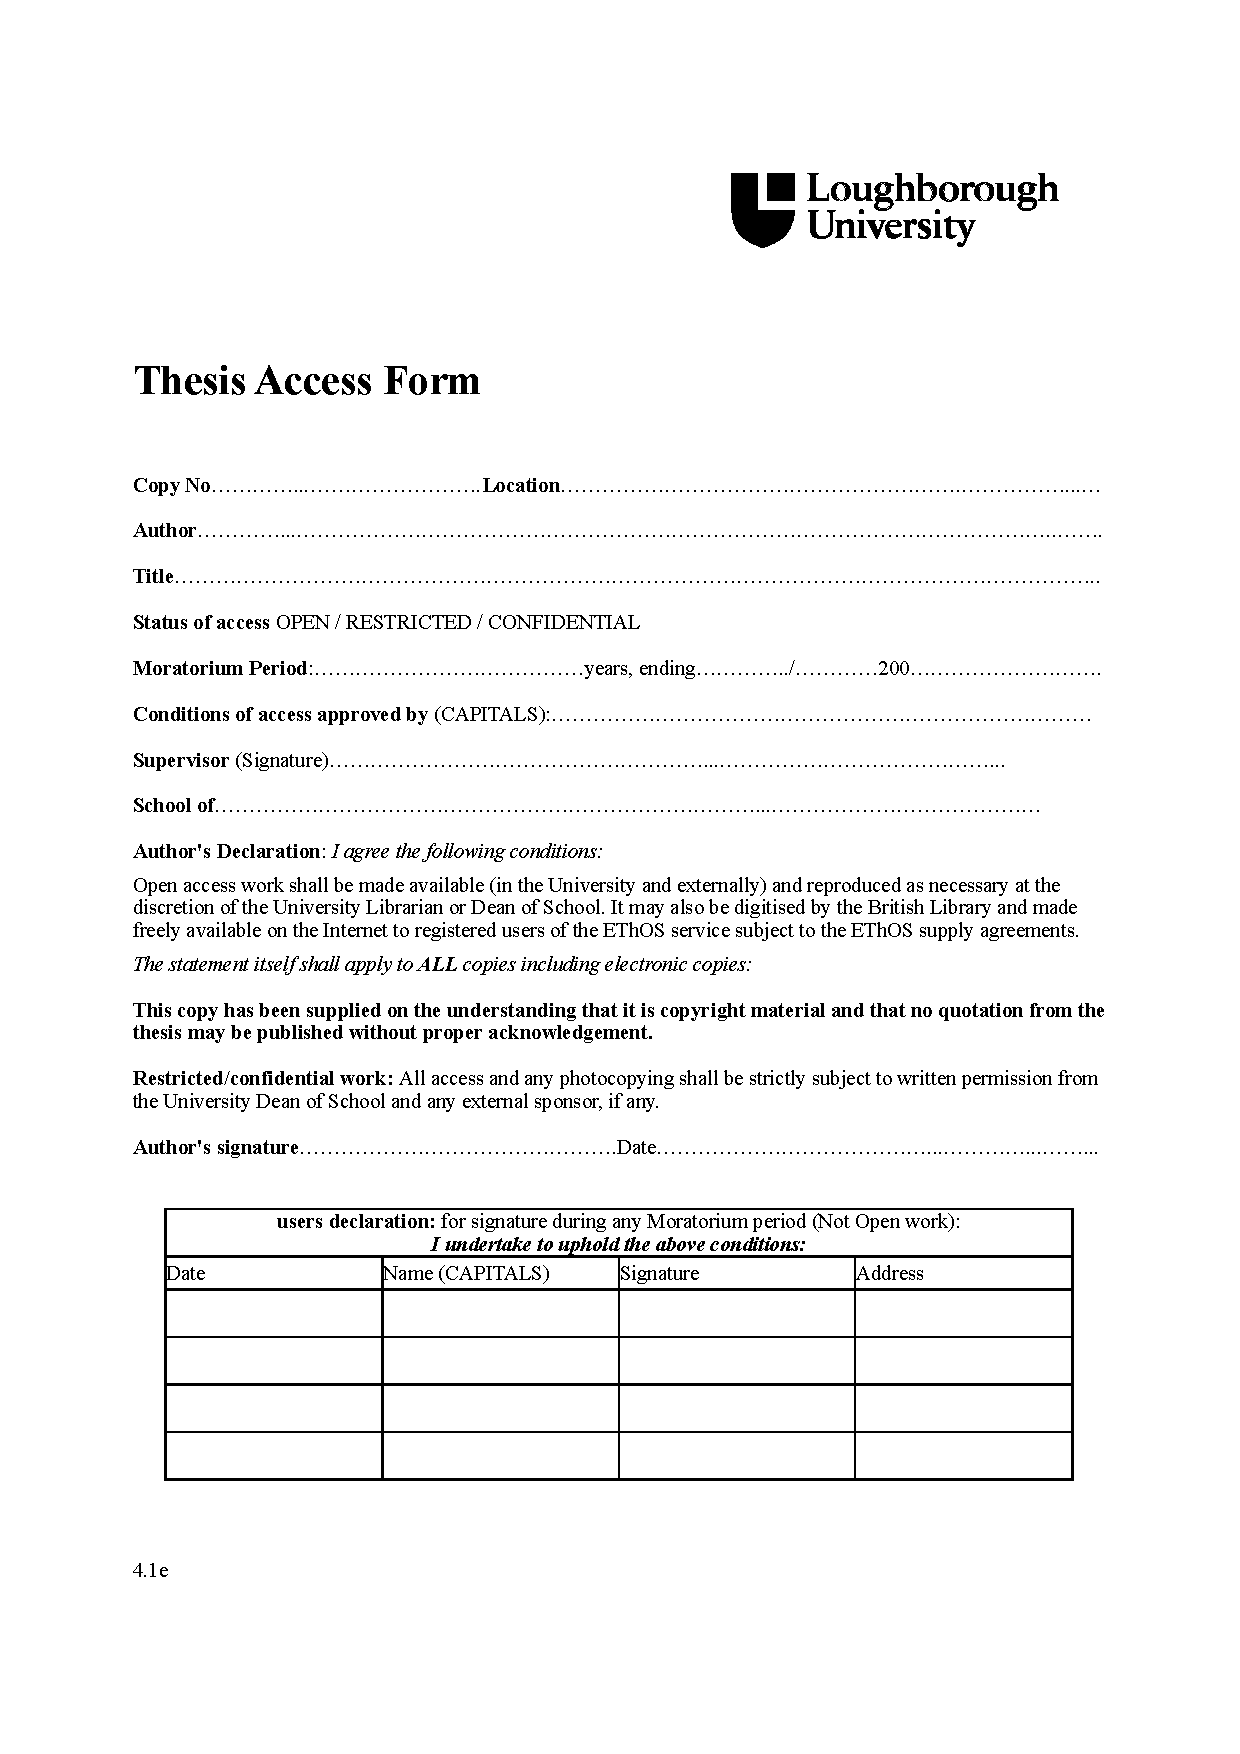
\includepdf[pages=1, pagecommand=, templatesize={5in}{10in}]{Front/LU/access.pdf}
% % Certificate of Originality
% 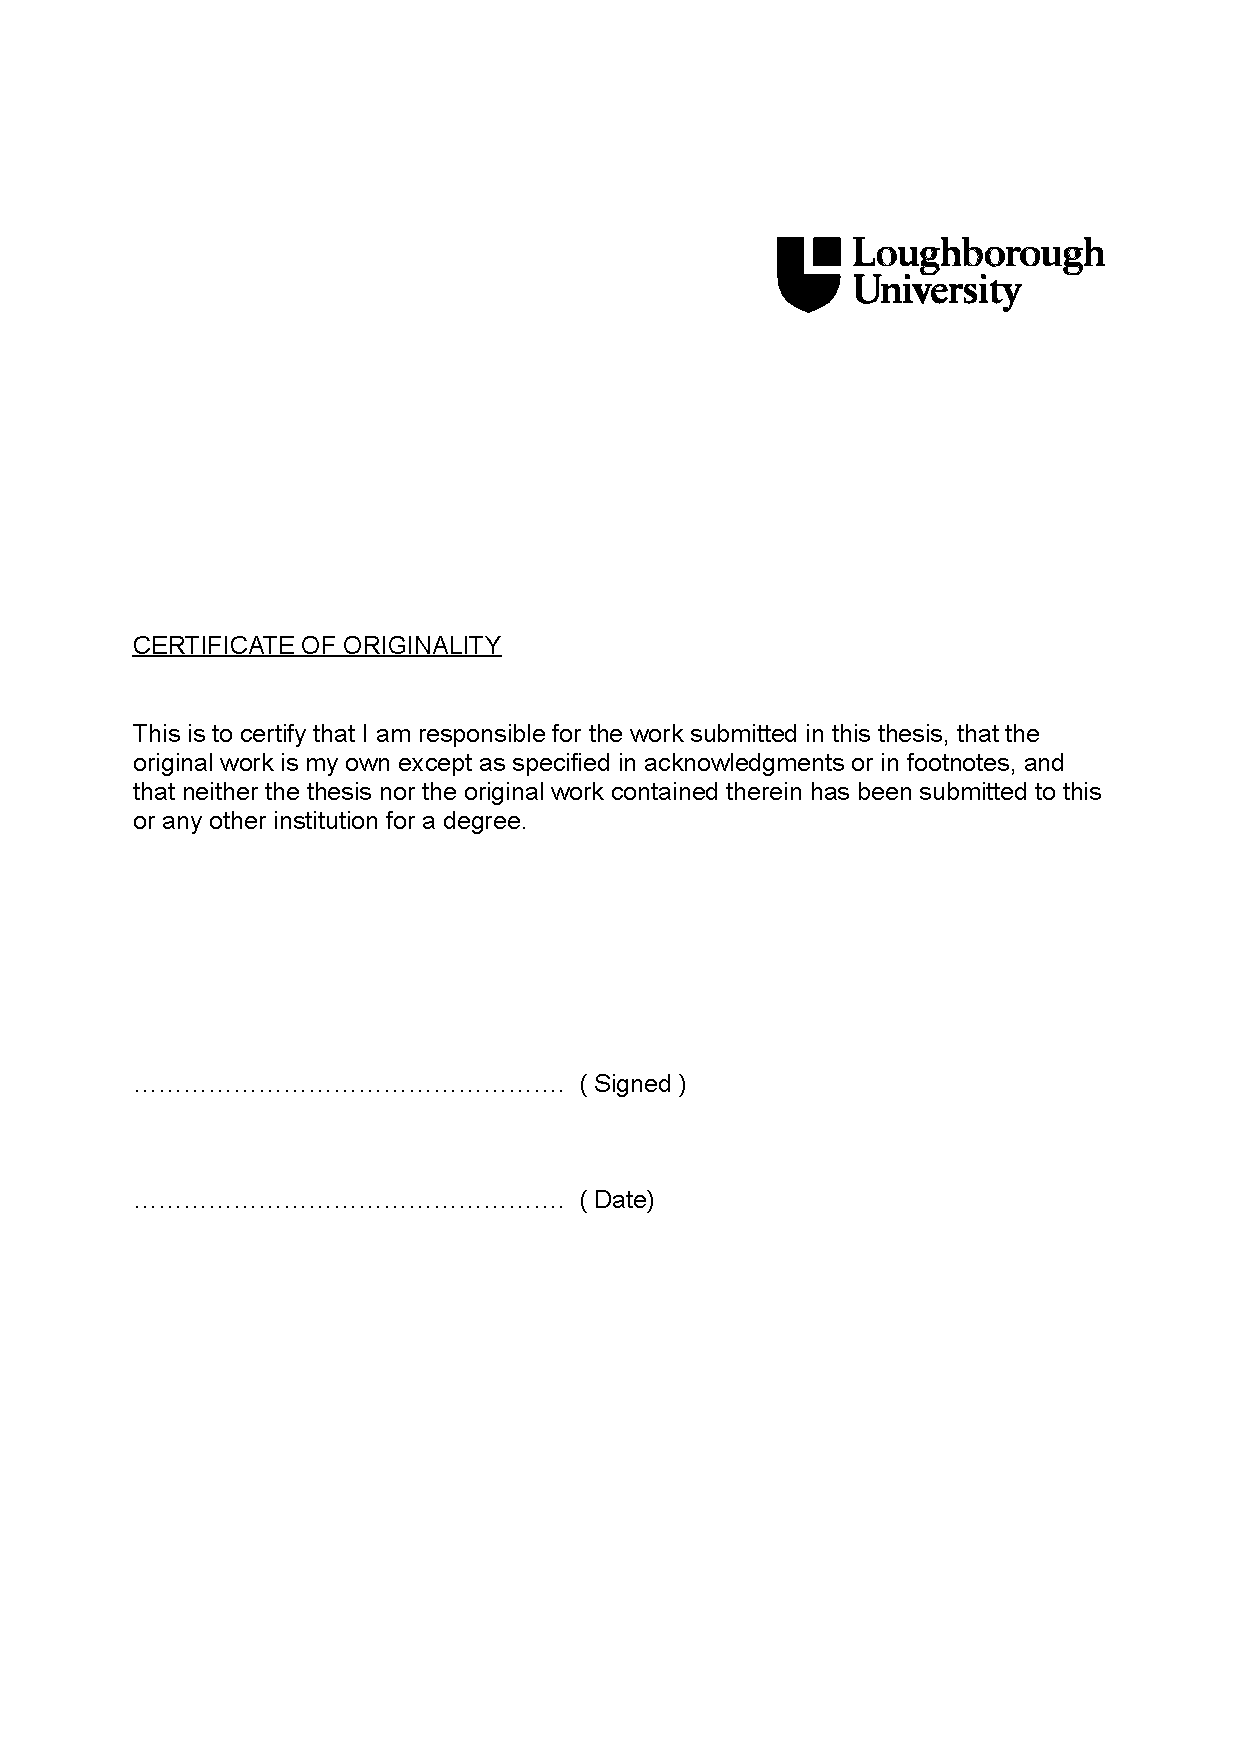
\includepdf[pages=-, pagecommand=, templatesize={5in}{10in}]{Front/LU/origin.pdf}

% Abstract
\addcontentsline{toc}{chapter}{Abstract}
\chapter*{Abstract}
In this coursework, I implement a JPEG Image Compression Simulation using MATLAB as frontend GUI and Python as backend JPEG CODEC. There are 2 simulation parameters $K$ and $Q'$ in the application. 
Several specific design considerations are introduced to the implementation, inclding an end-to-end MATLAB interface, an "Video Compression" functionality and DCT as Matrix Computation.
I conclude that both $K$ and $Q'$ can significantly affect the quality of the compressed image.


% % Acknowledgements
% \addcontentsline{toc}{chapter}{Acknowledgements}
% \chapter*{Acknowledgements}
% Acknowledgement section.

% Set the depth for your table of content
% Currently set at 2 (Chapter, Section, Subsection)
\setcounter{tocdepth}{2}
% Include a table of content
\tableofcontents

% Include a list of figures
\addcontentsline{toc}{chapter}{List of Figures}
\listoffigures

% Include a list of tables
\addcontentsline{toc}{chapter}{List of Tables}
\listoftables

% Include a list of Listings
\addcontentsline{toc}{chapter}{List of Listings}
\renewcommand*{\lstlistlistingname}{List of Listings}
\lstlistoflistings

% Include a list of abbreviations using nomenclature package
%\addcontentsline{toc}{chapter}{List of Abbreviations}
%\printnomenclature[3cm] 

\newpage

% Set page numbering to arabic for body of Thesis
\pagenumbering{arabic}


% To keep everything neat I included each chapter as a separate .tex file
% Each contains a single chapter, they include all the settings defined in this .tex file
% Allows easier moving around of chapters

% Use \include{<path to .tex file>} to include documents
% For example
\chapter{Introduction}
\label{chap:introduction}

This project is based on a mobile robot that has been built with latest AI technology and various sensor capabilities.
It could be programmed in Python.
It has a latest Realsense camera from Intel, which could capture both colour RGB image and depth image and be processed with a Nvidia nano board which supports image processing and deep learning. 
It also has multiple proximity sensors at its front, sides and back.

The task we have done in this project is programming its behaviours and test them to see if it works fully functionally. There are two types of behaviour we have been working on, Reactive Behaviours and Following Behaviours.

\subsection{Reactive Behaviours}
In this part we have designed robot’s behaviour simulate Braitenberg’s vehicle behaviour. 
There are four different behaviours: Love, Fear, Aggression as long as curious. 
We have used a black backpack as our targeted object and used deep learning to train the robot using its camera to recognize that specific backpack in a complex environment. 
When the robot has detected the targeted object, it will initiate the behaviour that we have been assigned.

\subsection{Following Behaviours}
In this part we programmed the robot to follow a human that has been detected by its RGBD camera and not only follow its movement, but also keep a safe distance from targeted human. 

For each behaviour, aspects of assumptions, system design, implementation and test \& analysis are described in details.






\chapter{More Examples}
\label{chap:examples}

\section{Subfigures}
\begin{figure*}[ht!]
    \centering
    \begin{subfigure}[b]{0.67\textwidth}
        \centering
        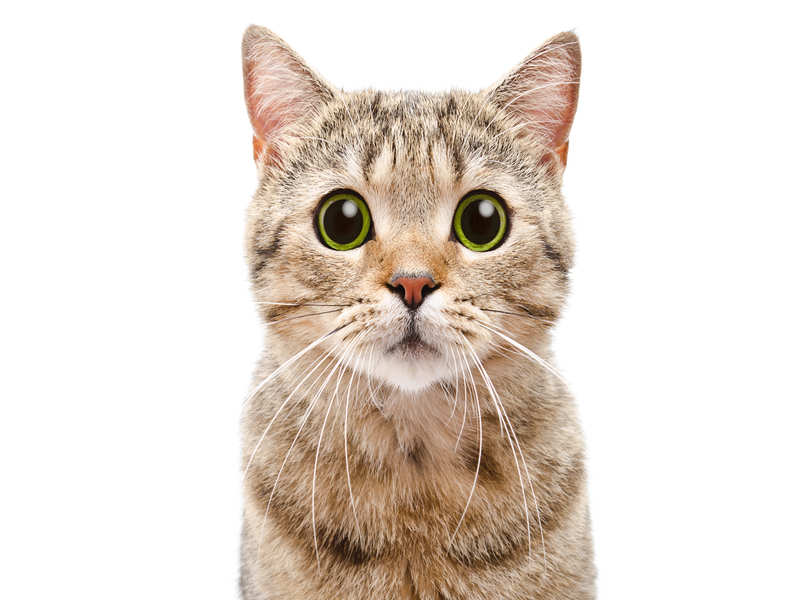
\includegraphics[width=\linewidth]{cat}
        \caption{Figure 1}
    \end{subfigure}
    \hfill
    \begin{minipage}[b]{0.3\textwidth}
	    \begin{subfigure}[b]{\linewidth}
	        \centering
	        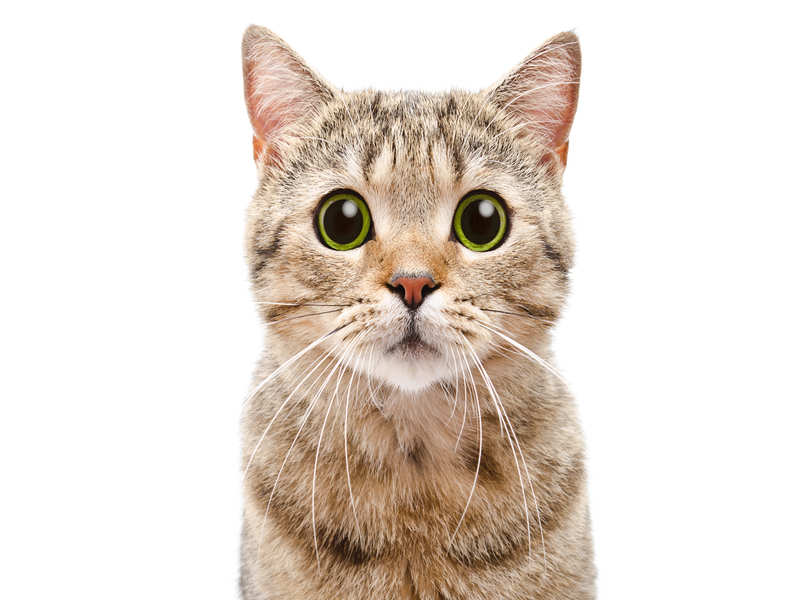
\includegraphics[width=\linewidth]{cat}
	        \caption{Figure 2}
	    \end{subfigure}
	    \\
	    \begin{subfigure}[b]{\linewidth}
	        \centering
	        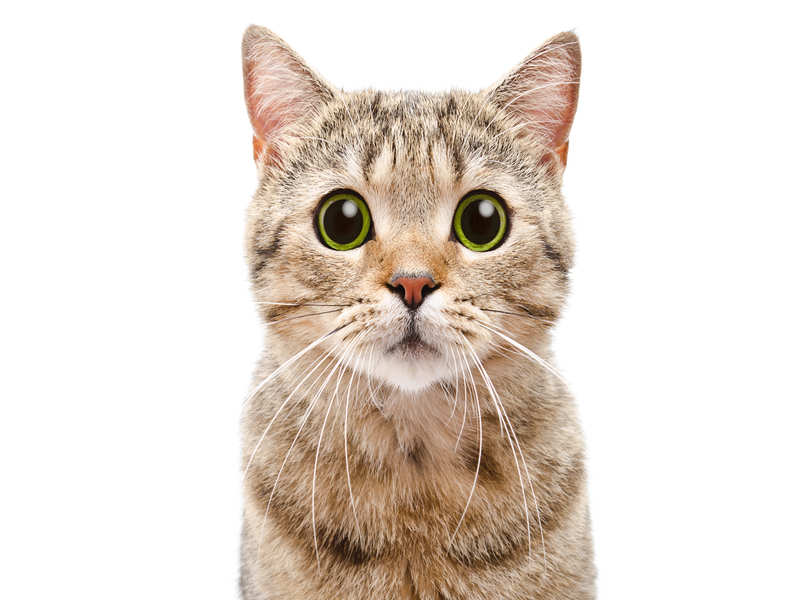
\includegraphics[width=\linewidth]{cat}
	        \caption{Figure 3}
	    \end{subfigure}
	\end{minipage}
    \caption{Subfigures in One Figure (1).}
    \label{fig:subfigures-1}
\end{figure*}

\begin{figure*}[ht!]
    \centering
    \begin{subfigure}[b]{0.67\textwidth}
        \centering
        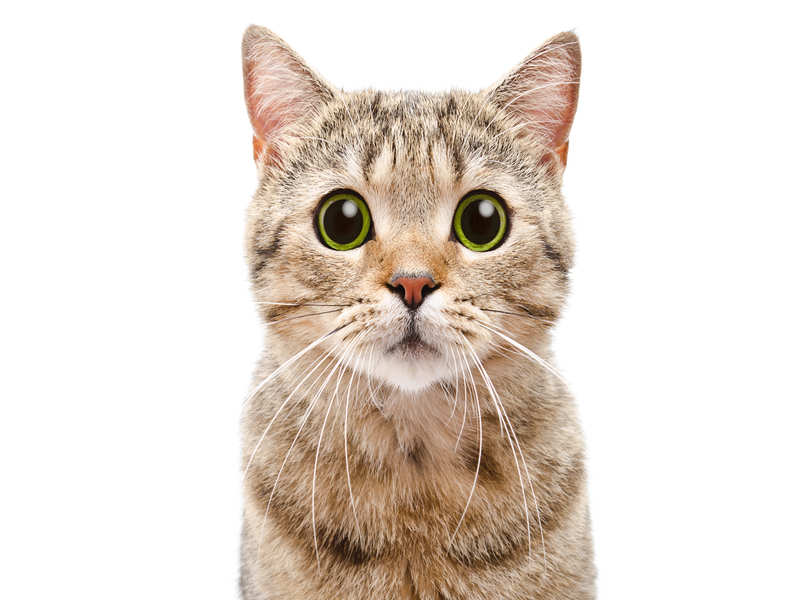
\includegraphics[width=\linewidth]{cat}
        \caption{Figure 1}
    \end{subfigure}
    ~
    \begin{subfigure}[b]{0.67\textwidth}
        \centering
        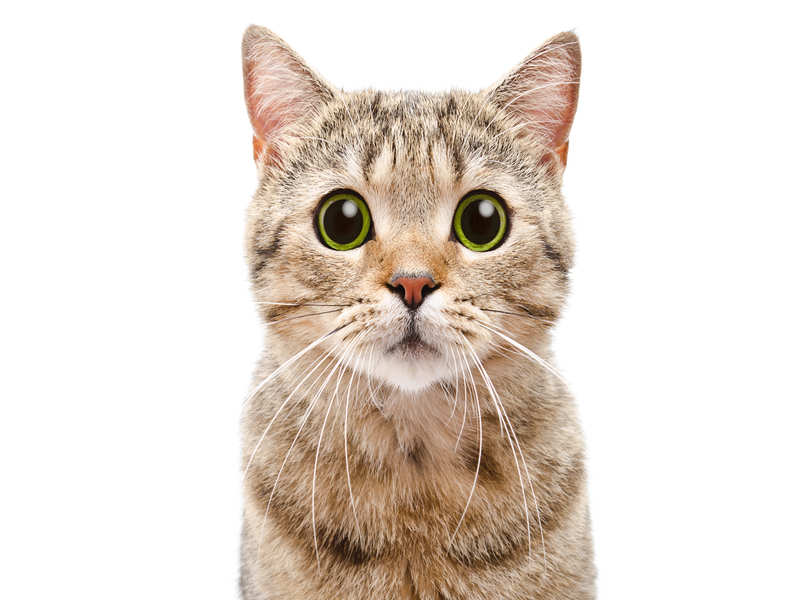
\includegraphics[width=\linewidth]{cat}
        \caption{Figure 2}
    \end{subfigure}
    \caption{Subfigures in One Figure (2).}
    \label{fig:subfigures-2}
\end{figure*}

\section{Landscape Page}

\begin{landscape}
\scriptsize{
\begin{longtable}[]{@{}lllll@{}}
\toprule
Subnet & IPv4 Address / Prefix & IPv4 Address Range & IPv6
Address / Prefix & IPv6 Address Range\tabularnewline
\midrule
\endhead
\texttt{BT-R001} - \texttt{BT001} & \texttt{23.0.0.0/28} &
\texttt{23.0.0.1} - \texttt{23.0.0.14} & \texttt{2001:2300:0:0::/64} &
\texttt{2001:2300:0:0::1} -
\texttt{2001:2300:0:0:ffff:ffff:ffff:fffe}\tabularnewline
\texttt{BT-R002} - \texttt{BT002} & \texttt{23.0.0.16/28} &
\texttt{23.0.0.17} - \texttt{23.0.0.30} & \texttt{2001:2300:0:1::/64} &
\texttt{2001:2300:0:1::1} -
\texttt{2001:2300:0:1:ffff:ffff:ffff:fffe}\tabularnewline
\texttt{BT-R003} - \texttt{BT003} & \texttt{23.0.0.32/28} &
\texttt{23.0.0.33} - \texttt{23.0.0.62} & \texttt{2001:2300:0:2::/64} &
\texttt{2001:2300:0:2::1} -
\texttt{2001:2300:0:2:ffff:ffff:ffff:fffe}\tabularnewline
\texttt{BT-R001} - \texttt{BT-R002} & \texttt{23.0.0.48/30} &
\texttt{23.0.0.49} - \texttt{23.0.0.50} & \texttt{2001:2300:0:3::/64} &
\texttt{2001:2300:0:3::1} -
\texttt{2001:2300:0:3:ffff:ffff:ffff:fffe}\tabularnewline
\texttt{BT-R002} - \texttt{BT-R003} & \texttt{23.0.0.52/30} &
\texttt{23.0.0.53} - \texttt{23.0.0.54} & \texttt{2001:2300:0:4::/64} &
\texttt{2001:2300:0:4::1} -
\texttt{2001:2300:0:4:ffff:ffff:ffff:fffe}\tabularnewline
\texttt{BT-R001} - \texttt{BT-R003} & \texttt{23.0.0.56/30} &
\texttt{23.0.0.57} - \texttt{23.0.0.58} & \texttt{2001:2300:0:5::/64} &
\texttt{2001:2300:0:5::1} -
\texttt{2001:2300:0:5:ffff:ffff:ffff:fffe}\tabularnewline
\texttt{BT-R002} - \texttt{DT} & \texttt{23.0.0.60/30} &
\texttt{23.0.0.61} - \texttt{23.0.0.62} & \texttt{2001:2300:0:6::/64} &
\texttt{2001:2300:0:6::1} -
\texttt{2001:2300:0:6:ffff:ffff:ffff:fffe}\tabularnewline
\texttt{BT-R003} - \texttt{Virgin} & \texttt{56.0.0.60/30} &
\texttt{56.0.0.61} - \texttt{56.0.0.62} & \texttt{2001:5600:0:6::/64} &
\texttt{2001:5600:0:6::1} -
\texttt{2001:5600:0:6:ffff:ffff:ffff:fffe}\tabularnewline
\texttt{BT-R003} - \texttt{Central} & \texttt{100.100.2.0/30} &
\texttt{100.100.2.1} - \texttt{100.100.2.2} & &\tabularnewline
\bottomrule
\caption{Allocation of IPv4 and IPv6 Addresses to Subnets in BT Network.}
\label{tab:ip}
\end{longtable}
}

\scriptsize{
\begin{longtable}[]{@{}lllllll@{}}
\toprule
Connection & Interface 1 & IPv4 Address & IPv6 Address & Interface 2 & IPv4 Address & IPv6
Address \tabularnewline
\midrule
\endhead
\texttt{BT-R001} - \texttt{BT001} & \texttt{BT-R001}:
\texttt{FastEthernet0/1/0} & \texttt{23.0.0.1} &
\texttt{2001:2300:0:0::1} & \texttt{BT001}: \texttt{eth0} &
\texttt{23.0.0.2} & \texttt{2001:2300:0:0::2}\tabularnewline
\texttt{BT-R002} - \texttt{BT002} & \texttt{BT-R002}:
\texttt{FastEthernet0/1/0} -\textgreater{} \texttt{Vlan\ 1} &
\texttt{23.0.0.17} & \texttt{2001:2300:0:1::1} & \texttt{BT002}:
\texttt{eth0} & \texttt{23.0.0.18} &
\texttt{2001:2300:0:1::2}\tabularnewline
\texttt{BT-R003} - \texttt{BT003} & \texttt{BT-R003}:
\texttt{FastEthernet0/1/0} -\textgreater{} \texttt{Vlan\ 2} &
\texttt{23.0.0.33} & \texttt{2001:2300:0:2::1} & \texttt{BT003}:
\texttt{eth0} & \texttt{23.0.0.34} &
\texttt{2001:2300:0:2::2}\tabularnewline
\texttt{BT-R001} - \texttt{BT-R002} & \texttt{BT-R001}:
\texttt{FastEthernet0/0} & \texttt{23.0.0.49} &
\texttt{2001:2300:0:3::1} & \texttt{BT-R002}: \texttt{FastEthernet0/0} &
\texttt{23.0.0.50} & \texttt{2001:2300:0:3::2}\tabularnewline
\texttt{BT-R002} - \texttt{BT-R003} & \texttt{BT-R002}:
\texttt{FastEthernet0/1} & \texttt{23.0.0.53} &
\texttt{2001:2300:0:4::1} & \texttt{BT-R003}: \texttt{FastEthernet0/1} &
\texttt{23.0.0.54} & \texttt{2001:2300:0:4::2}\tabularnewline
\texttt{BT-R001} - \texttt{BT-R003} & \texttt{BT-R001}:
\texttt{FastEthernet0/1} & \texttt{23.0.0.57} &
\texttt{2001:2300:0:5::1} & \texttt{BT-R003}: \texttt{FastEthernet0/0} &
\texttt{23.0.0.58} & \texttt{2001:2300:0:5::2}\tabularnewline
\texttt{BT-R002} - \texttt{DT} & \texttt{BT-R002}:
\texttt{FastEthernet0/1/1} -\textgreater{} \texttt{Vlan\ 3} &
\texttt{23.0.0.61} & \texttt{2001:2300:0:6::1} & \texttt{DT} &
\texttt{23.0.0.62} & \texttt{2001:2300:0:6::2}\tabularnewline
\texttt{BT-R003} - \texttt{Virgin} & \texttt{BT-R003}:
\texttt{FastEthernet0/1/2} -\textgreater{} \texttt{Vlan\ 4} &
\texttt{56.0.0.62} & \texttt{2001:5600:0:6::2} & \texttt{Virgin} &
\texttt{56.0.0.61} & \texttt{2001:5600:0:6::1}\tabularnewline
\texttt{BT-R003} - \texttt{Central} & \texttt{BT-R003}:
\texttt{FastEthernet0/1/1} -\textgreater{} \texttt{Vlan\ 5} &
\texttt{100.100.2.2} & & \texttt{Central} & \texttt{100.100.2.1}
&\tabularnewline
\bottomrule
\caption{Interfaces for Each Physical Connection and Corresponding IPv4 and IPv6 Addresses.}
\label{tab:interfaces}
\end{longtable}
}

\end{landscape}

% \include{Chapter/Requirements}
% \include{Chapter/Design}
% \include{Chapter/Testing}
% \chapter{Conclusions}
\label{chap:discussion}

% In this project we have successfully developed and tested two behaviours for our robot. 
% The first one is Reactive behaviour, which we refer to Braitenberg’s four behaviours, ‘ Love’, ‘Curious’, ‘Aggression’, ‘Fear’. We made our robot able to act four different behaviour regarding to a targeted object, a backpack. The robot itself are able to wonder around the lab and looking for the backpack, after it gather the targeted object in its camera, it will execute the behaviour that we have assigned to it. 
% We have designed a following behaviour to our robot as well, robot will firstly choose a human to follow, analysis that human’s details and then start to follow him in a desire distance, it will turn its direction as well. We also add interrupt function, which means even another person come in through the testing, even fully block the person that robot firstly chosen, robot will still be able to recognize the initial target and still follow that target.

In this coursework, both Reactive Behaviours and Following Behaviours of mobile robot are designed and implemented.
The robot with Reactive Behaviours mimics Braitenberg behaviors, more specifically love, aggression, fear and curiosity.
The robot first wanders around the environment to locate the object of interest (backpack in this case). Once the object is located, a  Braitenberg behavior is performed by the robot.

The robot with Following Behaviours keeps following the designated person on the scene while keeping a safe distance.
The robot first wanders around the environment to locate the person of interest.
Once the designated person is located, the robot moves toward the person while maintaining a safe distance.
In the scenario of possible hijacking by another person, the robot distinguishes between the two persons and only follows the person with the highest similarity score.

Testing procedures are proposed and performed on both tasks. The testing results show that our design and implementation is correct and robust.



% Include a Chapter names References to the table of content
\addcontentsline{toc}{chapter}{References}
% Rename Bibliography to References
\renewcommand\bibname{References}
\bibliography{Bib/tex}

% Include authors publications and appendix section
% \addcontentsline{toc}{chapter}{Publications}
\chapter*{Publications}
\label{chap:Publications}

% Author publication section
% If not using the references per chapter option you need to include the bibliography inline
% This was done by creating a bibtex file containing the publications and including in a separate LaTeX file, using \nocite{*} this includes all bibtex items, generating the .bbl file and then copying and pasting below.

List of authors academic publications

\begingroup
% Remove title and space of header for this chapter
\titleformat{\chapter}[display]
    {\normalfont\huge\bfseries}{\chaptertitlename\ \thechapter}{20pt}{\Huge}
\titlespacing*{\chapter}{0pt}{0pt}{-80pt}
\renewcommand\bibname{}
\begin{thebibliography}{1}

%\bibitem{}

\end{thebibliography}
\endgroup

% To include copies of the publications use the includepdf package and point to .pdf files of papers
% Example
%\includepdf[pages=-, pagecommand=, templatesize={5in}{10in}]{Publications/Pubs/le1_biothreads.pdf}

% Appedix
\appendix

\begingroup

\chapter{Source Code}
\label{app:code}


\section{JPEG CODEC Code in Python}
\label{app:sec:python}

\subsection{Python-MATLAN Interface \texttt{matlab.py}}
\lstinputlisting[caption={Code of Python-MATLAN Interface \texttt{matlab.py}.},captionpos=t,language=Python]{Code/matlab.py}


\endgroup


\end{document}
